\documentclass[a4paper, oneside]{article}
\usepackage[utf8]{inputenc}
\usepackage[ngerman]{babel}
\usepackage[top=2.5cm, bottom=3cm, outer=2.5cm, inner=2.5cm, heightrounded]{geometry}
\usepackage{graphicx}
\usepackage{morefloats}
\usepackage{wrapfig}
\usepackage{hyperref}
\usepackage{cite}
\usepackage{siunitx}
\usepackage[default]{sourcesanspro}
\usepackage[T1]{fontenc}
\usepackage{url}
\usepackage{marginnote}
\usepackage[font=footnotesize]{caption}
\usepackage{color}
\usepackage{xcolor}
\usepackage{multicol}
\usepackage[fleqn]{mathtools}
\usepackage{amssymb}
\usepackage{wrapfig}
\usepackage[noindentafter]{titlesec}
\usepackage{fancyhdr}
\usepackage{lastpage}
\usepackage{comment}

%% LÖSUNGEN ANZEIGEN
\newif\ifshow
%\showtrue
\showfalse

%%%SECTIONING
\renewcommand*{\marginfont}{\noindent\rule{0pt}{0.7\baselineskip}\footnotesize}

\newcommand{\aufgabe}[1]{\subsection{#1}}
\newcommand{\loesung}[1]{\subsubsection{#1}}

\newcommand{\simpleset}[1]{\ensuremath \left\{ #1 \right\}}
\newcommand{\ematrix}[2]{\renewcommand{\arraystretch}{1}\ensuremath\left(\begin{array}{@{}#1@{}}#2\end{array}\right)}

\renewcommand{\theenumi}{\alph{enumi})}
\renewcommand{\labelenumi}{\text{\theenumi}}

\newcounter{aufgabe}
%\newenvironment{lsg}{\loesung}{}
\ifshow
  \newenvironment{lsg}{\loesung}{}
\else
  \excludecomment{lsg}
\fi

\newenvironment{inhalt}
  {\paragraph{Inhalt des Übungsblatts:}\itemize\let\origitem\item}
  {\enditemize\vspace{2em}}

\newcommand{\R}{\ensuremath\mathbb{R}}
\newcommand{\N}{\ensuremath\mathbb{N}}
\newcommand{\Z}{\ensuremath\mathbb{Z}}
\newcommand{\LM}{\ensuremath\mathbb{L}}
\newcommand{\intd}{\ensuremath\mathrm{d}}
\newcommand{\e}{\ensuremath\mathrm{e}}
\renewcommand{\d}{\,\mathrm{d}}
\newcommand{\stf}[1]{\ensuremath \left[ #1 \right]}

\newcommand{\cas}{\hfill (CAS)}
\newcommand{\seite}[1]{\textit{(S. #1)}}

\newcommand{\vektor}[1]{\ensuremath\begin{pmatrix} #1 \end{pmatrix}}


\everymath{\displaystyle}

%Malpunkte
\mathcode`\*="8000
{\catcode`\*\active\gdef*{\cdot}}

%SECTION
\titleformat{\section}
{\clearpage\setcounter{aufgabe}{0}\vspace{1em}\Large\raggedright\bfseries}
{}
{0pt}
{}

\titleformat{\subsection}[runin]
{\stepcounter{aufgabe}\vspace{1px}\normalfont\raggedright\bfseries}
{A\theaufgabe: }
{0pt}
{\ }

\titleformat{\subsubsection}[runin]
{\normalfont\raggedright\bfseries}
{Lösung \theaufgabe: }
{0pt}
{\ }


%FANCYHDR
\pagestyle{fancy}
\lhead{\small Simon König\\ Joshua Fabian}
\rhead{\small Mathecrashkurs 2018}
\cfoot{Seite \thepage\thinspace von\thinspace\pageref{LastPage}}
\lfoot{}
\renewcommand{\headrulewidth}{0.5pt}
\renewcommand{\footrulewidth}{0pt}

\title{Mathe-Crashkurs 2018 - Übungsblatt}
\date{\today}
\author{Simon König, Joshua Fabian}

\chead{\Large Übungsblatt 4}

\begin{document}
\begin{inhalt}
	\item Zufallsexperimente \seite{81}
	\item Kombinatorik \seite{85}, Binomalverteilung und Bernoulli-Versuch \seite{87}
	\item Hypothesentest \seite{89}
	\item Vermischtes
\end{inhalt}

\aufgabe{Kombinatorik und Pfadregeln: }
Ein Fußballspieler verwandelt erfahrungsgemäß $90\%$ aller Elfmeter.
\begin{enumerate}
	\item Mit welcher Wahrscheinlichkeit verwandelt er von drei Elfmetern nur den ersten bzw. mindestens einen?
	\item Für ein Ereignis $C$ gilt: $P(C)=\binom{40}{x}*0,9^y+z^8$ Gib geeignete Werte für $x,y$ und $z$ an. Beschreibe $C$ in Worten.
\end{enumerate}
\begin{lsg}{}
	\begin{enumerate}
		\item \begin{align*}
			&p_1=\frac 9{10}*\frac1{10}^2=0,009=0,9\%\\
			&p_2=\underbrace{\frac 9 {10}*\frac 1{10}^2}_{\text{1 Treffer}}
						+\underbrace{3* \frac 9 {10}^2*\frac 1{10}}_{\text{2 Treffer}}
						+\underbrace{\frac 9 {10}^3}_{\text{3 Treffer}} = 0,981=98,1\%
					\end{align*}
		\item $x$ bzw $y$ ist die Anzahl der Treffer:$x=y=32=40-8$ und $z$ ist die Gegenwahrscheinlichkeit: $z=0,1=1-0,9$

		$P(C)$ ist die Wahrscheinlichkeit dafür, dass der Fußballer $32$ von $40$ Elfmetern mit einer Wahrscheinlichkeit von $0,9$ trifft, also $32$ Treffer bei $40$ Versuchen.
	\end{enumerate}
\end{lsg}


\aufgabe{Hypothesentest 1: }
Ein Labor entwickelt einen neuen Impfstoff und testet ihn in einem Tierversuch mit 800 Mäusen. Mit dem Impfstoff dürfen keine klinischen Studien an Menschen durchgeführt werden, wenn sich im Tierversuch mindestens $2\%$ unerwünschte Nebenwirkungen zeigen.
\begin{enumerate}
	\item Bestimme für die Nullhypothese $H_0:p\geq 2^\%$ die Entscheidungsregel für den Test mit 800 Mäusen mit einer Irrtumswahrscheinlichkeit von höchstens $1\%$.
	\item Welche Bedeutung haben die Fehler 1. und 2. Art? Wie könnte man erreichen, dass sowohl der Fehler 1. Art als auch der Fehler 2. Art gleichzeitig kleiner werden?
\end{enumerate}
\begin{lsg}{}
	\begin{enumerate}
		\item \begin{align*}
			&n=800, \alpha=0,01, H_0:p\geq 2\%
			\intertext{$X$ ist die Anzahl Mäuse mit Nebenwirkungen, $X$ ist binomialverteilt. Gesucht ist ein $k$ für das gilt:}
			B_{800;0,02}\quad &P(X\leq k)\leq 0,01\\
			&P(X\leq 7)=0,0095\\
			&P(X\leq 8)=0,021
			\intertext{Damit bildet $7$ die Grenze des Annahmebereichs.}
			&A=\simpleset{0,1,\ldots,7}\\
			&\overline A =\simpleset{8,\ldots,800}
			\intertext{Wenn mehr als 7 Mäuse Nebenwirkungen zeigen, ist $H_0$ zu verwerfen.}
		\end{align*}
		\item Der Fehler 1. Art ist die Wahrscheinlichkeit, mit der man durch Zufall eine wahre Hypothese fälschlicherweise verwirft, der Fehler 2. Art ist die Wahrscheinlichkeit, mit der man eine falsche Hypothese fälschlicherweise annimmt.

		Beide Fehler bekommt man nur durch Erhöhung des Versuchsumfangs $n$ kleiner. Somit fallen Zufälle, die zu den Fehlern führen weniger stark ins Gewicht.
	\end{enumerate}
\end{lsg}


\aufgabe{Hypothesentest 2: }
Ein Computerhersteller bezieht von einem Lieferanten Speicherchips. Erfahrungsgemäß sind $95\%$ der Chips einwandfrei. Wenn mindestens $95\%$ der Chips einwandfrei sind, nimmt er die Lieferung an, ansonsten schickt er sie zurück.

Stelle eine Entscheidungsregel auf, wenn bei einem Stichprobenumfang von 200 Chips die Irrtumswahrscheinlichkeit höchstens $10\%$ betragen soll.
\begin{lsg}{}
	\begin{align*}
		&n=200, p=0.95, H_0:p\geq 0.95, \alpha=0.1
		\intertext{$X$ ist die Anzahl einwandfreier Chips, $X$ ist binomialverteilt.}
		B_{200;0,95}\quad & P(X\leq k )\leq 0,1\\
		&P(X\leq 185)=0,0781\\
		&P(X\leq 186)=0,1299
		\intertext{Damit bildet 186 die Grenze des Annahmebereichs.}
		&A=\simpleset{186,187,\ldots,200}\\
		&\overline A =\simpleset{1,\ldots,185}
		\intertext{Wenn mehr als 185 Chips einwandfrei sind, so behält er die Sendung, sonst schickt er sie zurück.}
	\end{align*}
\end{lsg}


\aufgabe{Hypothesentest 3: }
Bei einem Glücksspiel wird ein Tetraeder mit den Tahlen 1 bis 4 eingeetzt. Eva behauptet, der Tetraeder sei nicht ideal, er liefere mit einer Wahrscheinlichkeit von höchstens $15\%$ eine 4. Daraufhin wirft Tim mit dem Tetraeder 60 mal und notiert sich, wie oft die Zahl 4 auftritt. Er erhält insgesamt 12 mal die Zahl 4.

Kann Tim bei einem Signifikanzniveau von $6\%$ die Behauptung von Eva widerlegen? Führe einen geeigneten Signifikanztest durch.

\begin{lsg}{}
	\begin{align*}
		&n=60, H_0:p_4\geq 15\%, \alpha=0.06
		\intertext{$X$ ist die Anzahl geworfener 4er, $X$ ist binomialverteilt.}
		B_{60;0,15}\quad & P(X\geq k )\leq 0,06\\
		&P(X\geq 13)=0,106\\
		&P(X\geq 14)=0,0578
		\intertext{Damit bildet 13 die Grenze des Annahmebereichs.}
		&A=\simpleset{0,1,\ldots,13}\\
		&\overline A =\simpleset{14,\ldots,60}
		\intertext{Das heißt, Tim kann die Behauptung nicht widerlegen, denn 12 liegt nicht in $A$.}
	\end{align*}
\end{lsg}


\clearpage

\aufgabe{Wiederholung: }
\begin{enumerate}
	\item Gegeben sei folgende Funktion: $F(x,y)=2x^3-5y+x^2+10x-10$. Bestimmen Sie die Ableitung der durch $F(x,y)=0$ implizit gegebenen Funktion $y=h(x)$.
	\item Gegeben sind die Funktionen:
	$f(x) = (u \circ v)(x)$ und $g(x) = (u* v)(x)$
	Bestimme die Ableitungen von $f$ und $g$ für $u(x)=x^2$ und $v(x)=\sin(2x)$
	\item Bestimme jeweils $f_i'(3)$
	\begin{multicols}{2}
		\begin{itemize}
			\item $f_1(x) = (x+5)^2$
			\item $f_2(x) = \frac{1}{(x-5)^2}$
		\end{itemize}
	\end{multicols}
	\item Gegeben sei die Funktion $f(x) = \frac{1-4x^2}{x^2}$. Ihr Schaubild ist $K$, wo schneidet die Tangente an $P(1|f(1))$ die $x$-Achse?
\end{enumerate}
\begin{lsg}{}
	\begin{enumerate}
		\item Aus $F(x,y)=0$ und $y=h(x)$ folgt:\begin{alignat*}{2}
		&2x^3-5y+10x-10=0\quad&&|\ \text{Nach $y=$ umformen}\\
		&y=\frac{2}{5} x^3+\frac{1}{5} x^2+2x-2 &&\Rightarrow h(x)\\
		&h'(x)=\frac{6}{5} x^2+\frac{2}{5}x+2
		\end{alignat*}
		\item \begin{align*}
		f'(x)&=\left(u(v(x))\right)'=\left({\sin(2x)}^2\right)'=2\sin(2x)\cdot \cos(2x) \cdot 2=4\sin(2x)\cdot \cos(2x)\\
		g'(x)&=(u(x)\cdot v(x))'=\left(x^2\cdot \sin(2x)\right)'=2x\cdot \sin(2x)+x^2\cdot 2\cos(2x)
		\end{align*}
		\item \begin{align*}
		f_1'(x)&=2(x+5)&\Rightarrow  &f_1'(3)=16\\
		f_2'(x)&=\frac{-2}{(x-5)^3}&\Rightarrow &f_2'(3)=\frac{1}{4}
		\end{align*}
		\item Aufstellen der allgemeinen Tangentengleichung für $f$:
		\begin{align*}
			t_f(x)&=f'(x_0)*(x-x_0)+f(x_0)\\
						&=\left(\frac{-2}{x_0^3}\right)*(x-x_0)+\frac{1}{x_0^2}-4\\
			\intertext{Für $x_0=1$ folgt:}
			t_{f,1}&=-2(x-1)-3\\
			\intertext{Finden der Nullstelle von $t_{f,1}$:}
			t_{f,1}&\overset!=0=-2(x-1)-3\\
		\end{align*}
	\end{enumerate}
\end{lsg}



\aufgabe{Wiederholung: } (vgl. Abitur 2015)
\begin{multicols}{2}
	Die Abbildung zeigt den Graphen der Ableitungsfunktion $f'$ einer ganzrationalen Funktion $f$.
	Entscheide ob die folgenden Aussagen wahr oder falsch sind. Begründe jeweils Deine Antwort.
	\begin{enumerate}
		\item Der Graph von $f$ hat bei $x=-3$ einen Tiefpunkt.
		\item $f(-2)<f(-1)$
		\item $f''(-2)+f'(-2)<1$
		\item Der Grad der Funktion $f$ ist mindestens vier.
	\end{enumerate}
	\columnbreak
	\centering
	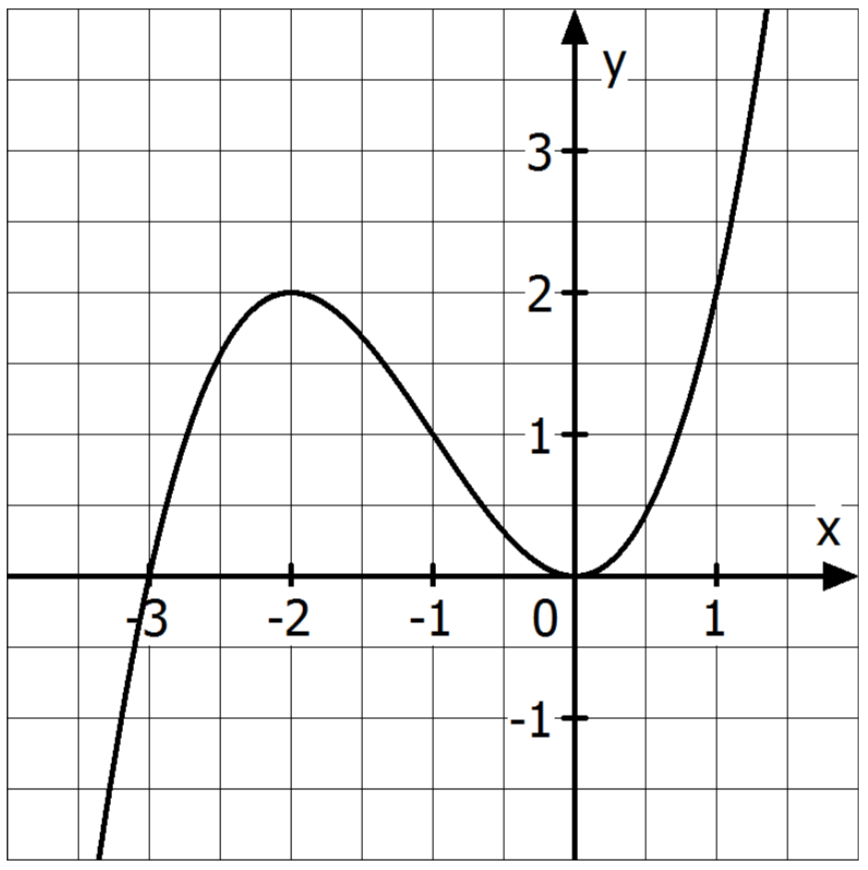
\includegraphics[width=0.7\linewidth]{Graphanalyse.png}
\end{multicols}
\begin{lsg}{}
	\begin{enumerate}
		\item Wahr, Vorzeichenwechsel bei $x=-3$
		\item Wahr, streng monoton steigend im Intervall $[-2;-1]$
		\item Falsch, $f''(-2)+f'(-2)=0+2>1$
		\item Wahr, $f'$ besitzt zwei Extrempunkte $\rightsquigarrow f''$ ist mindestens vom Grad 2. Der Graph der Abbildung könnte auch drei Nullstellen haben, $f'$ ist also mindestens vom Grad 3.
	\end{enumerate}
\end{lsg}




\aufgabe{Wiederholung: } Bestimme die Lage der Geraden zueinander und ggf. den Schnittwinkel der beiden Geraden $g$ und $h$:
\begin{equation*}
	g: \vec x = \vektor{2\\2\\-3} + r*\vektor{2\\1\\-1} \text{ und } h: \vec x = \vektor{3\\0\\-1} + s* \vektor{1\\-2\\2}
\end{equation*}
\begin{lsg}{}
	Geraden sind nicht parallel, da die Richtungsvektoren nicht vielfache voneinander sind. Probe auf Schnittpunkt oder windschief:

	Gleichsetzen der Geradengleichungen ergibt mit $s=-1$ den Schnittpunkt $S(2|2|-3)$.

	Schnittwinkel:
	\begin{align*}
		&\angle \vektor{2\\1\\-1}, \vektor{1\\-2\\2}=\alpha\\
		\alpha &= \arccos\frac{\left|\vektor{2\\1\\-1}* \vektor{1\\-2\\2}\right|}{\sqrt{2^2+1+1}*\sqrt{1+2^2+2^2}}=\arccos\frac{2}{\sqrt{6}*3}=74,21^\circ
	\end{align*}
\end{lsg}

\end{document}
